\documentclass[compress,table,xcolor=table]{beamer}
\input{beamer_mirror.tex}
\begin{document}
% ------------------------------------------------------------------------------
\title{Implementing a general-purpose reflection API}
% - Intro ----------------------------------------------------------------------
\section{Introduction}
\begin{frame}
  \frametitle{Intro}
  \framesubtitle{What is this? Why am I here? Who are these people?}
  \makebox[\linewidth][c]{
    \begin{minipage}{\dimexpr\textwidth\relax}
    \centering
    
\includegraphics[
        width=0.9\textwidth,
        keepaspectratio
    ]{look_into_mirror.png}
    \end{minipage}
  }
\end{frame}
% ------------------------------------------------------------------------------
\begin{frame}
  \frametitle{Contents}
  \Large
  \begin{itemize}
    \item Reflection \smaller and \say{un-reflection}
    \item Metaobjects and metadata
    \item Reflection APIs
    \item Examples
    \item Some use-cases
  \end{itemize}
\end{frame}
% ------------------------------------------------------------------------------
\begin{frame}
  \frametitle{Metaobject}
  \larger
  \begin{itemize}
    \item A {\em meta-level} representation of a {\em base-level} entity
      \begin{itemize}
      \smaller
        \item namespace, type, function, constructor, destructor, variable,
          constant, expression, \ldots
      \end{itemize}
    \item On the {\em meta-level\footnote{unlike the base-level}} all
      of the above are \say{reified}
      \begin{itemize}
      \smaller
        \item can be stored in variables, used as function arguments and
          return values,
        \item provide the ability to write reflection algorithm libraries,
        \item working at compile-time.
      \end{itemize}
    \item We say a metaobject \say{reflects} the {\em base-level} entity
  \end{itemize}
\end{frame}
% ------------------------------------------------------------------------------
\begin{frame}
  \frametitle{Metaobject}
  \framesubtitle{continued}
  \larger
  \begin{itemize}
    \item Provides access to {\em metadata} describing the reflected
      {\em base-level} entity
      \begin{itemize}
      \smaller
        \item type of a variable,
        \item data members of a \inlinecode{struct},
        \item constructors or member functions of a \inlinecode{class},
        \item base classes of a \inlinecode{class},
        \item return type of a function,
        \item parameters of a function,
        \item enumerators in an \inlinecode{enum} type,
        \item name of a namespace, type, function, data member, parameter, etc.
        \item address of a variable, data member or member function,
        \item specifiers like \inlinecode{virtual}, \inlinecode{constexpr},
          \inlinecode{static}, \inlinecode{noexcept}, \inlinecode{public},
          \inlinecode{protected}, \inlinecode{private}, etc.
        \item source location\footnote{except for built-ins},
        \item \ldots
      \end{itemize}
  \end{itemize}
\end{frame}
% ------------------------------------------------------------------------------
\begin{frame}[fragile]
  \frametitle{Metaobject}
  \framesubtitle{continued}
  \larger
  In a program a {\em metaobject} is a compile-time constant
    {\larger value} of a type satisfying the~following concept:
  \begin{lstlisting}[language=c++2x]
template <typename X>
concept metaobject = (*@{\em not-really-important-here}@*);
  \end{lstlisting}
  \vfill
  Can be used to constrain function arguments:
  \begin{lstlisting}[language=c++2x]
void foo((*@\listinghl{metaobject}@*) auto m) { /*...*/ }
  \end{lstlisting}
  or more generally in a \inlinecode{requires} clause,
  \begin{lstlisting}[language=c++2x]
void bar(auto m)
  requires((*@\listinghl{metaobject}@*)<decltype(m)> &&
           something_else(m)) {
    /*...*/
}
  \end{lstlisting}
\end{frame}
% ------------------------------------------------------------------------------
\begin{frame}[fragile]
  \frametitle{Reflection}
  \larger
  \begin{itemize}
    \item The process of obtaining metadata or metaobjects providing metadata
      indirectly
    \item Done through a~dedicated operator or~language expression
    \item For example
  \end{itemize}
  \begin{lstlisting}[language=c++2x]
const auto meta_int = (*@\listinghl{mirror}\footnote{\inlinecode{mirror} is a~placeholder
      for the~actual reflection expression}@*)(int);
static_assert(
  metaobject<decltype(meta_int)>);
  \end{lstlisting}
\end{frame}
% ------------------------------------------------------------------------------
\begin{frame}
  \frametitle{\say{Un-reflection}}
  \framesubtitle{a.k.a \say{splicing}}
  \larger
  \begin{itemize}
    \item The reverse of reflection
    \item Getting back to the base-level entity reflected by a metaobject
    \item As in\ldots
    \begin{itemize}
      \smaller
      \item getting a type,
      \item getting the value of a constant,
      \item getting the pointer or reference to a variable,
      \item getting the pointer to a function or a member function,
      \item invoking a function, constructor or operator,
      \item etc.
    \end{itemize}
    \item \ldots through an operation on a metaobject reflecting that
      {\em base-level} entity
    \item \say{Splicing} can also mean emitting a snippet of code involving
      base-level entities, reflected by metaobjects
  \end{itemize}
\end{frame}
% ------------------------------------------------------------------------------
\begin{frame}
  \frametitle{Reflection API}
  \larger
  \begin{itemize}
    \item Set of (compile-time) functions operating on {\em metaobjects}
    \item Several groups
    \begin{itemize}
      \item metaobject classification functions,
      \item primitive metadata extraction,
      \item metaobject sequence operations,
      \item general-purpose algorithms,
      \item predicates, comparators, transformation functions,
      \item syntax sugar, placeholder expressions,
      \item \ldots
    \end{itemize}
  \item Are \inlinecode{consteval} (or \inlinecode{constexpr})\footnote{
      assumed, but omitted from examples in here to save space on slides}
  \end{itemize}
\end{frame}
% - Design ---------------------------------------------------------------------
\section{API Design}
% ------------------------------------------------------------------------------
\begin{frame}
  \frametitle{Reflection API}
  \framesubtitle{design considerations}
  \larger
  \begin{itemize}
    \item The general API design stuff
    \item Concise and clear syntax, functional-style
    \item Support for as many use-cases as possible
    \item Provide functions handling recurring patterns and use-cases
    \item Support composition of function calls into bigger custom algorithms
    \item Proper ADL\footnote{argument-dependent lookup}; should not require
      excessive name qualification
    \item Be similar to the STL and other commonly-used libraries\footnote{
        boost, \ldots}, where it makes sense.
  \end{itemize}
\end{frame}
% ------------------------------------------------------------------------------
\begin{frame}[fragile]
  \frametitle{Hello, reflection!}
  \framesubtitle{the obligatory first example}
  \begin{lstlisting}[language=c++2x]
struct hello {};

int main() {
  hello world;

  std::cout << get_name((*@\listinghl{mirror}@*)(hello))
            << ", "
            << (*@\listinghl{get_name}@*)(mirror(world))
            << "!" << std::endl;

    return 0;
}
  \end{lstlisting}
\end{frame}
% ------------------------------------------------------------------------------
\begin{frame}
  \frametitle{Reflection API}
  \framesubtitle{metaobject classification functions}
  \begin{itemize}
    \item Indicate {\em \larger what} does a metaobject reflect
    \item Return \inlinecode{true} or \inlinecode{false}
    \item \inlinecode{auto reflects_object(metaobject auto m) -> bool;}
    \item \footnotesize\inlinecode{auto reflects_\{object_sequence, named, alias, typed,
    scope, scope_member, enumerator, record_member, base, namespace, global_scope,
    type, enum, record, class, lambda, constant, variable, lambda_capture,
    function_parameter, callable, function, member_function,
    special_member_function, constructor, destructor, operator, conversion_operator,
    expression, parenthesized_expression, function_call_expression\}(metaobject auto m) -> bool;}
    \item \normalsize Typically used in \inlinecode{requires} clauses or
      in \inlinecode{if constexpr}
  \end{itemize}
\end{frame}
% ------------------------------------------------------------------------------
\begin{frame}
  \frametitle{Reflection API}
  \framesubtitle{metadata retrieval functions}
  \begin{itemize}
    \item Return individual \say{atomic} pieces of metadata
    \item Some are applicable to all metaobjects
    \begin{itemize}
      \smaller
      \item \inlinecode{get_source_line}, \inlinecode{get_source_column},
        \inlinecode{reflects_same}, \ldots
    \end{itemize}
  \item Some only on metaobjects reflecting specific {\em base-level} entities
    \begin{itemize}
      \smaller
      \item where they make sense,
      \item \inlinecode{get_name}, \inlinecode{get_type}, \inlinecode{get_scope},
        \inlinecode{get_enumerators}, \ldots
    \end{itemize}
  \end{itemize}
\end{frame}
% ------------------------------------------------------------------------------
\begin{frame}
  \frametitle{Reflection API}
  \framesubtitle{metadata retrieval functions}
  \larger
  \begin{itemize}
  \item Return one of these things:
    \begin{itemize}
      \smaller
      \item boolean values (\inlinecode{is_static}),
      \item integer values (\inlinecode{get_source_line}),
      \item other constant values\footnote{like enumerators} (\inlinecode{get_constant}),
      \item pointers or references\footnote{to values, data member, functions},
      \item strings\footnote{string views actually} (\inlinecode{get_source_file_name},
        \inlinecode{get_name}),
      \item types\footnote{or type identity} (\inlinecode{get_reflected_type},
      \item other metaobjects (\inlinecode{get_scope}, \inlinecode{get_data_members}).
    \end{itemize}
  \end{itemize}
\end{frame}
% ------------------------------------------------------------------------------
\begin{frame}[fragile]
  \frametitle{Reflection API}
  \framesubtitle{somewhere in logging\ldots}
  \begin{lstlisting}[language=c++2x,basicstyle=\scriptsize\ttfamily]
auto get_display_name(metaobject auto mo) -> string_view
  requires((*@\listinghl{reflects_named}@*)(mo));
  \end{lstlisting}
  \begin{lstlisting}[language=c++2x,basicstyle=\footnotesize\ttfamily]
void log_who_did_this(
  metaobject auto mo,
  ostream& log) {
  if constexpr((*@\listinghl{reflects_global_scope}@*)(mo)) {
    log << "it was the global scope!"
  } else if constexpr((*@\listinghl{reflects_named}@*)(mo)) {
    log << "it was " << get_display_name(mo);
  } else {
    log << "how the hell should I know?"
  }
}
  \end{lstlisting}
\end{frame}
% - Primitives -----------------------------------------------------------------
\section{Primitives}
% ------------------------------------------------------------------------------
\begin{frame}[fragile]
  \frametitle{Metadata getters}
  \framesubtitle{source location}
  \begin{lstlisting}[language=c++2x]
auto get_source_file_name(metaobject auto)
  -> string_view;
  \end{lstlisting}
  \vfill
  \begin{lstlisting}[language=c++2x,basicstyle=\footnotesize\ttfamily]
auto get_source_line(metaobject auto)
  -> unsigned long;
  \end{lstlisting}
  \vfill
  \begin{lstlisting}[language=c++2x,basicstyle=\footnotesize\ttfamily]
auto get_source_column(metaobject auto)
  -> unsigned long;
  \end{lstlisting}
\end{frame}
% ------------------------------------------------------------------------------
\begin{frame}[fragile]
  \frametitle{Metadata getters}
  \framesubtitle{names}
  \begin{lstlisting}[language=c++2x]
auto get_name(metaobject auto mo)
  -> string_view
  requires(reflects_named(mo));
// "basic_string"
  \end{lstlisting}
  \vfill
  \begin{lstlisting}[language=c++2x]
auto get_display_name(metaobject auto mo)
  -> string_view
  requires(reflects_named(mo));
// "string"
  \end{lstlisting}
  \vfill
  \begin{lstlisting}[language=c++2x]
auto get_full_name(metaobject auto mo)
  -> string;
// "std::basic_string<char, ...>"
  \end{lstlisting}
\end{frame}
% ------------------------------------------------------------------------------
\begin{frame}[fragile]
  \frametitle{Metadata getters}
  \framesubtitle{specifiers}
  \begin{lstlisting}[language=c++2x,basicstyle=\footnotesize\ttfamily]
auto is_constexpr(metaobject auto mo) -> bool
  requires(reflects_variable(mo) ||
           reflects_callable(mo));
  \end{lstlisting}
  \vfill
  \begin{lstlisting}[language=c++2x,basicstyle=\footnotesize\ttfamily]
auto is_noexcept(metaobject auto mo) -> bool
  requires(reflects_callable(mo));
  \end{lstlisting}
  \vfill
  \begin{lstlisting}[language=c++2x,basicstyle=\footnotesize\ttfamily]
auto is_explicit(metaobject auto mo) -> bool
  requires(reflects_constructor(mo) ||
           reflects_conversion_operator(mo));
  \end{lstlisting}
  \vfill
  \begin{lstlisting}[language=c++2x,basicstyle=\footnotesize\ttfamily]
auto is_static(metaobject auto mo) -> bool
  requires(reflects_variable(mo) ||
           reflects_member_function(mo));
  \end{lstlisting}
  \vfill
  \begin{lstlisting}[language=c++2x,basicstyle=\footnotesize\ttfamily]
auto is_virtual(metaobject auto mo) -> bool
  requires(reflects_base(mo) ||
           reflects_destructor(mo)) ||
           reflects_member_function(mo));
  \end{lstlisting}
\end{frame}
% ------------------------------------------------------------------------------
\begin{frame}[fragile]
  \frametitle{Metadata getters}
  \framesubtitle{miscelaneous}
  \begin{lstlisting}[language=c++2x,basicstyle=\scriptsize\ttfamily]
auto is_scoped_enum(metaobject auto mo) -> bool
  requires(reflects_type(mo));
  \end{lstlisting}
  \vfill
  \begin{lstlisting}[language=c++2x,basicstyle=\footnotesize\ttfamily]
auto uses_class_key(metaobject auto mo) -> bool
  requires(reflects_type(mo));
  \end{lstlisting}
  \vfill
  \begin{lstlisting}[language=c++2x,basicstyle=\footnotesize\ttfamily]
auto uses_default_copy_capture(metaobject auto mo)
  -> bool
  requires(reflects_lambda(mo));
  \end{lstlisting}
  \vfill
  \begin{lstlisting}[language=c++2x,basicstyle=\footnotesize\ttfamily]
auto is_explicitly_captured(metaobject auto mo)
  -> bool
  requires(reflects_lambda_capture(mo));
  \end{lstlisting}
  \vfill
  \begin{lstlisting}[language=c++2x,basicstyle=\footnotesize\ttfamily]
auto has_default_argument(metaobject auto mo) -> bool
  requires(reflects_function_parameter(mo));
  \end{lstlisting}
\end{frame}
% ------------------------------------------------------------------------------
\begin{frame}[fragile]
  \frametitle{Metadata getters}
  \framesubtitle{miscelaneous}
  \begin{lstlisting}[language=c++2x,basicstyle=\scriptsize\ttfamily]
auto has_lvalueref_qualifier(metaobject auto mo) -> bool
  requires(reflects_member_function(mo));
  \end{lstlisting}
  \vfill
  \begin{lstlisting}[language=c++2x,basicstyle=\footnotesize\ttfamily]
auto is_implicitly_declared(metaobject auto mo)
  -> bool
  requires(reflects_special_member_function(mo));
  \end{lstlisting}
  \vfill
  \begin{lstlisting}[language=c++2x,basicstyle=\footnotesize\ttfamily]
auto is_deleted(metaobject auto mo) -> bool
  requires(reflects_callable(mo));
  \end{lstlisting}
  \vfill
  \begin{lstlisting}[language=c++2x,basicstyle=\footnotesize\ttfamily]
auto is_defaulted(metaobject auto mo) -> bool
  requires(reflects_special_member_function(mo));
  \end{lstlisting}
  \vfill
  \begin{lstlisting}[language=c++2x,basicstyle=\footnotesize\ttfamily]
auto is_move_constructor(metaobject auto mo) -> bool
  requires(reflects_constructor(mo));
  \end{lstlisting}
\end{frame}
% ------------------------------------------------------------------------------
\begin{frame}[fragile]
  \frametitle{Metadata getters}
  \framesubtitle{constants and values}
  \begin{lstlisting}[language=c++2x,basicstyle=\small\ttfamily]
auto get_constant(metaobject auto mo)
  -> const auto
  requires(reflects_constant(mo));
  \end{lstlisting}
  \vfill
  \begin{lstlisting}[language=c++2x,basicstyle=\small\ttfamily]
auto get_value(metaobject auto mo)
  -> const auto&
  requires(reflects_variable(mo));
  \end{lstlisting}
  \vfill
  \begin{lstlisting}[language=c++2x,basicstyle=\small\ttfamily]
auto get_value(metaobject auto mo, auto& obj)
  -> const auto&
  requires(reflects_record_member(mo) &&
           reflects_variable(mo));
  \end{lstlisting}
\end{frame}
% ------------------------------------------------------------------------------
\begin{frame}[fragile]
  \frametitle{Metadata getters}
  \framesubtitle{references and pointers}
  \begin{lstlisting}[language=c++2x,basicstyle=\footnotesize\ttfamily]
auto get_reference(metaobject auto mo)
  -> auto&
  requires(reflects_variable(mo));
  \end{lstlisting}
  \vfill
  \begin{lstlisting}[language=c++2x,basicstyle=\footnotesize\ttfamily]
auto get_reference(metaobject auto mo, auto& obj)
  -> auto&
  requires(reflects_record_member(mo) &&
           reflects_variable(mo));
  \end{lstlisting}
  \vfill
  \begin{lstlisting}[language=c++2x,basicstyle=\footnotesize\ttfamily]
auto get_pointer(metaobject auto mo)
  -> auto*
  requires(reflects_variable(mo) ||
           reflects_function(mo));
  \end{lstlisting}
  \vfill
  \begin{lstlisting}[language=c++2x,basicstyle=\footnotesize\ttfamily]
auto get_pointer(metaobject auto mo, auto& obj)
  -> auto*
  requires(reflects_record_member(mo) &&
           reflects_variable(mo));
  \end{lstlisting}
\end{frame}
% ------------------------------------------------------------------------------
\begin{frame}[fragile]
  \frametitle{Metadata getters}
  \framesubtitle{invocation of callables}
  \begin{lstlisting}[language=c++2x,basicstyle=\footnotesize\ttfamily]
auto invoke(metaobject auto mo, auto&&... args)
  requires(reflects_member_function(mo) &&
           is_static(mo));
  \end{lstlisting}
  \vfill
  \begin{lstlisting}[language=c++2x,basicstyle=\footnotesize\ttfamily]
auto invoke(auto mo, auto& inst, auto&&... args)
  requires(reflects_member_function(mo) &&
           !is_static(mo));
  \end{lstlisting}
  \vfill
  \begin{lstlisting}[language=c++2x,basicstyle=\footnotesize\ttfamily]
auto invoke(metaobject auto mo, auto&&... args)
  requires(reflects_constructor(mo));
  \end{lstlisting}
  \vfill
  \begin{lstlisting}[language=c++2x,basicstyle=\footnotesize\ttfamily]
auto invoke_on(auto mo, auto& inst, auto&&... args)
  requires(reflects_member_function(mo));
  \end{lstlisting}
\end{frame}
% ------------------------------------------------------------------------------
\begin{frame}[fragile]
  \frametitle{Metadata getters}
  \framesubtitle{metaobjects}
 \begin{lstlisting}[language=c++2x,basicstyle=\small\ttfamily]
auto get_scope(metaobject auto mo)
  requires(reflects_scoped(mo));
  \end{lstlisting}
  \vfill
  \begin{lstlisting}[language=c++2x,basicstyle=\small\ttfamily]
auto get_type(metaobject auto mo)
  requires(reflects_typed(mo));
  \end{lstlisting}
  \vfill
  \begin{lstlisting}[language=c++2x,basicstyle=\small\ttfamily]
auto get_underlying_type(metaobject auto mo)
  requires(reflects_enum(mo));
  \end{lstlisting}
  \vfill
  \begin{lstlisting}[language=c++2x,basicstyle=\small\ttfamily]
auto get_aliased(metaobject auto mo)
  requires(reflects_alias(mo));
  \end{lstlisting}
  \vfill
  \begin{lstlisting}[language=c++2x,basicstyle=\small\ttfamily]
auto get_class(metaobject auto mo)
  requires(reflects_base(mo));
  \end{lstlisting}
  \vfill
  \begin{lstlisting}[language=c++2x,basicstyle=\footnotesize\ttfamily]
auto get_subexpression(metaobject auto mo)
  requires(reflects_parenthesized_expression(mo));
  \end{lstlisting}
\end{frame}
% ------------------------------------------------------------------------------
\begin{frame}[fragile]
  \frametitle{Metadata getters}
  \framesubtitle{{\em base-level} types}
 \begin{lstlisting}[language=c++2x,basicstyle=\small\ttfamily]
template <metaobject MO>
using get_reflected_type_t = (*@\listinghl{unspecified}@*);
  \end{lstlisting}
  \vfill
  \begin{lstlisting}[language=c++2x,basicstyle=\small\ttfamily]
auto get_reflected_type(metaobject auto mo)
  -> type_identity<(*@\listinghl{unspecified}@*)>
  requires(reflects_type(mo));
  \end{lstlisting}
  \vfill
  \begin{lstlisting}[language=c++2x,basicstyle=\small\ttfamily]
template <typename T>
auto is_type(
  metaobject auto mo,
  type_identity<T> = {})
  -> bool requires(reflects_type(mo));
  \end{lstlisting}
  \vfill
  \begin{lstlisting}[language=c++2x,basicstyle=\small\ttfamily]
template <template <typename> class Trait>
auto has_type_trait(metaobject auto mo) 
  -> bool requires(reflects_type(mo));
  \end{lstlisting}
\end{frame}
% - Sequences ------------------------------------------------------------------
\section{Sequences}
% ------------------------------------------------------------------------------
\begin{frame}
  \frametitle{Metaobject sequences}
  \larger
  \begin{itemize}
    \item Are (special kind of) metaobjects themselves
    \item Represent collections of other metaobjects
    \item Returned by many metaobject operations
    \begin{itemize}
      \smaller
      \item base classes,
      \item data members,
      \item member functions,
      \item constructors, destructors,
      \item enumerators,
      \item \ldots
    \end{itemize}
    \item Initially the metaobject elements of a sequence are not materialized
    \item Only \say{unpacked} if necessary to improve performance
  \end{itemize}
\end{frame}
% ------------------------------------------------------------------------------
\begin{frame}[fragile]
  \frametitle{Metaobject sequences}
  \framesubtitle{getting sequences}
  \begin{lstlisting}[language=c++2x,basicstyle=\small\ttfamily]
auto get_base_classes(metaobject auto mo)
  requires(reflects_class(mo));
  \end{lstlisting}
  \vfill
  \begin{lstlisting}[language=c++2x,basicstyle=\small\ttfamily]
auto get_captures(metaobject auto mo)
  requires(reflects_lambda(mo));
  \end{lstlisting}
  \vfill
  \begin{lstlisting}[language=c++2x,basicstyle=\small\ttfamily]
auto get_constructors(metaobject auto mo)
  requires(reflects_record(mo));
  \end{lstlisting}
  \vfill
  \begin{lstlisting}[language=c++2x,basicstyle=\small\ttfamily]
auto get_data_members(metaobject auto mo)
  requires(reflects_record(mo));
  \end{lstlisting}
  \vfill
  \begin{lstlisting}[language=c++2x,basicstyle=\small\ttfamily]
auto get_destructors(metaobject auto mo)
  requires(reflects_record(mo));
  \end{lstlisting}
\end{frame}
% ------------------------------------------------------------------------------
\begin{frame}[fragile]
  \frametitle{Metaobject sequences}
  \framesubtitle{getting sequences}
  \begin{lstlisting}[language=c++2x,basicstyle=\small\ttfamily]
auto get_enumerators(metaobject auto mo)
  requires(reflects_enum(mo));
  \end{lstlisting}
  \vfill
  \begin{lstlisting}[language=c++2x,basicstyle=\small\ttfamily]
auto get_member_functions(metaobject auto mo)
  requires(reflects_record(mo));
  \end{lstlisting}
  \vfill
  \begin{lstlisting}[language=c++2x,basicstyle=\small\ttfamily]
auto get_member_types(metaobject auto mo)
  requires(reflects_record(mo));
  \end{lstlisting}
  \vfill
  \begin{lstlisting}[language=c++2x,basicstyle=\small\ttfamily]
auto get_operators(metaobject auto mo)
  requires(reflects_record(mo));
  \end{lstlisting}
  \vfill
  \begin{lstlisting}[language=c++2x,basicstyle=\small\ttfamily]
auto get_parameters(metaobject auto mo)
  requires(reflects_callable(mo));
  \end{lstlisting}
\end{frame}
% ------------------------------------------------------------------------------
\begin{frame}
  \frametitle{Metaobject sequences}
  \framesubtitle{basic operations}
  \larger
  \begin{itemize}
    \item Is something a sequence (\inlinecode{is_object_sequence})
    \item Is there anything in the sequence (\inlinecode{is_empty})
    \item How many elements are there (\inlinecode{get_size})
    \item Get the I-th element (\inlinecode{get_element<I>})
    \item Concatenate\footnote{merge several sequences into one}
      (\inlinecode{concat})
    \item Flatten\footnote{transform a sequence of sequences into a single
      sequence}(\inlinecode{flatten})
  \end{itemize}
\end{frame}
% ------------------------------------------------------------------------------
\begin{frame}[fragile]
  \frametitle{Metaobject sequences}
  \framesubtitle{basic operations}
  \begin{lstlisting}[language=c++2x,basicstyle=\small\ttfamily]
auto is_object_sequence(auto mo) -> bool;
  \end{lstlisting}
  \vfill
  \begin{lstlisting}[language=c++2x,basicstyle=\small\ttfamily]
auto is_empty(auto mo) -> bool
  requires(is_object_sequence(mo));
  \end{lstlisting}
  \vfill
  \begin{lstlisting}[language=c++2x,basicstyle=\small\ttfamily]
auto get_size(auto mo) -> size_t
  requires(is_object_sequence(mo));
  \end{lstlisting}
  \vfill
  \begin{lstlisting}[language=c++2x,basicstyle=\small\ttfamily]
auto concat(auto... mo)
  requires((... && is_object_sequence(mo)));
  \end{lstlisting}
  \vfill
  \begin{lstlisting}[language=c++2x,basicstyle=\small\ttfamily]
auto flatten(auto mo)
  requires(is_object_sequence(mo));
  \end{lstlisting}
\end{frame}
% ------------------------------------------------------------------------------
\begin{frame}[fragile]
  \frametitle{Metaobject sequences}
  \framesubtitle{basic iteration}
  \begin{lstlisting}[language=c++2x,basicstyle=\small\ttfamily]
void for_each(auto mo, F function)
  requires(is_object_sequence(mo));
  \end{lstlisting}
  \begin{lstlisting}[language=c++2x]
(*@\listinghl{for_each}@*)(
  get_enumerators(mirror(weekday)),
  [](metaobject auto mo) {
    cout << get_name(mo)
         << ": "
         << int(get_constant(mo))
         << endl;
  });
  \end{lstlisting}
\end{frame}
% - Sugar ----------------------------------------------------------------------
\section{Sugar}
% ------------------------------------------------------------------------------
\begin{frame}
  \frametitle{Placeholder expressions}
  \larger
  \begin{itemize}
    \item Placeholders
    \begin{itemize}
      \item pre-defined constant objects -- \inlinecode{_1}, \inlinecode{_2}, \ldots
    \end{itemize}
    \item Placeholder expressions
    \begin{itemize}
      \item Functions matching the metaobject operations in name taking,
        placeholders or other placeholder expressions as arguments
    \end{itemize}
    \item Create objects (like lambdas) that can be called later
    \item Predicates, comparators, transformation functions
    \item Custom composite algorithms
  \end{itemize}
\end{frame}
% ------------------------------------------------------------------------------
\begin{frame}[fragile]
  \frametitle{Placeholder expressions}
  \framesubtitle{predicates}
  \begin{lstlisting}[language=c++2x,basicstyle=\small\ttfamily]
reflects_named(_1);
reflects_destructor(_1);
is_static(_1);
is_pure_virtual(_1);
is_public(_1);
is_noexcept(_1);
is_constexpr(_1);
is_copy_constructor(_1);
has_rvalueref_qualifier(_1);
uses_class_key(_1);
is_type<int>(get_type(_1));
has_type_trait<std::is_floating_point>(_1);
  \end{lstlisting}
\end{frame}
% ------------------------------------------------------------------------------
\begin{frame}[fragile]
  \frametitle{Placeholder expressions}
  \framesubtitle{comparators}
  \begin{lstlisting}[language=c++2x,basicstyle=\small\ttfamily]
reflects_same(_1, _2);
get_name(_1) < get_name(_2);
get_sizeof(_1) == get_sizeof(_2);
get_size(get_name(_1)) > get_size(get_name(_2));
  \end{lstlisting}
\end{frame}
% ------------------------------------------------------------------------------
\begin{frame}[fragile]
  \frametitle{Placeholder expressions}
  \framesubtitle{transforms}
  \begin{lstlisting}[language=c++2x,basicstyle=\small\ttfamily]
get_type(_1);
get_scope(_1);
get_display_name(_1);
get_name(get_aliased(_1));
get_name(get_aliased(get_type(_1)));
get_size(get_enumerators(_1));
is_empty(get_data_members(_1));
get_size(get_name(get_scope(get_type(_1))));
get_type(get_element<0>(get_operators(_1)));
get_name(get_element<1>(get_parameters(_1)));
  \end{lstlisting}
\end{frame}
% - Algorithms -----------------------------------------------------------------
\section{Algorithms}
% ------------------------------------------------------------------------------
\begin{frame}
  \frametitle{Algorithms}
  \larger
  \begin{itemize}
    \item Implement small specific, but non-trivial functionality
    \item On top of the primitive metaobject operations
    \item Can be easily combined in many ways into bigger, custom algorithms
    \item Can form and inter-operate with placeholder expressions
    \item Promote code re-usability
    \item Mostly operate on metaobject sequences
    \item \say{Un-reflection} can be done in the function objects passed
      to the algorithms
  \end{itemize}
\end{frame}
% ------------------------------------------------------------------------------
\begin{frame}[fragile]
  \frametitle{Algorithms}
  \framesubtitle{transform}
  Takes a sequence, returns new sequence containing metaobjects that are
  the result of applying a transformation \inlinecode{function}
  \begin{lstlisting}[language=c++2x]
auto (*@\listinghl{transform}@*)(auto mo, auto function)
  requires(is_object_sequence(mo));
  \end{lstlisting}
  \vfill
  \begin{lstlisting}[language=c++2x,basicstyle=\footnotesize\ttfamily]
auto get_base_class_types = (*@\listinghl{transform}@*)(
    get_base_classes(_1),
    (*@\listinghl{get_class}@*)(_1));

auto get_parameter_types = (*@\listinghl{transform}@*)(
    get_parameters(_1),
    (*@\listinghl{get_type}@*)(_1));
  \end{lstlisting}
\end{frame}
% ------------------------------------------------------------------------------
\begin{frame}[fragile]
  \frametitle{Algorithms}
  \framesubtitle{filter, remove-if}
  Takes a sequence, returns new sequence containing only metaobjects
  satisfying a \inlinecode{predicate}
  \begin{lstlisting}[language=c++2x]
auto (*@\listinghl{filter}@*)(auto mo, auto predicate)
  requires(is_object_sequence(mo));
  \end{lstlisting}
  \vfill
  Takes a sequence, returns new sequence containing only metaobjects
  {\em not} satisfying a \inlinecode{predicate}
  \begin{lstlisting}[language=c++2x]
auto (*@\listinghl{remove_if}@*)(auto mo, auto predicate)
  requires(is_object_sequence(mo));
  \end{lstlisting}
  \vfill
  \begin{lstlisting}[language=c++2x,basicstyle=\footnotesize\ttfamily]
auto get_virtual_functions =
  (*@\listinghl{filter}@*)(get_member_functions(_1), (*@\listinghl{is_virtual}@*)(_1));

auto get_nonstatic_members =
  (*@\listinghl{remove_if}@*)(get_data_members(_1), (*@\listinghl{is_static}@*)(_1));
  \end{lstlisting}
\end{frame}
% ------------------------------------------------------------------------------
\begin{frame}[fragile]
  \frametitle{Algorithms}
  \framesubtitle{count-if}
  Takes a sequence, returns the count of metaobjects satisfying
  a \inlinecode{predicate}
  \begin{lstlisting}[language=c++2x]
auto (*@\listinghl{count_if}@*)(auto mo, auto predicate)
  requires(is_object_sequence(mo));
  \end{lstlisting}
  \vfill
  \begin{lstlisting}[language=c++2x,basicstyle=\small\ttfamily]
auto count_public_bases =
  (*@\listinghl{count_if}@*)(
    get_base_classes(_1),
    is_public(_1));

auto count_integer_members =
  (*@\listinghl{count_if}@*)(
    get_data_members(_1),
    has_type_trait<is_integral>(get_type(_1)));
  \end{lstlisting}
\end{frame}
% ------------------------------------------------------------------------------
\begin{frame}[fragile]
  \frametitle{Algorithms}
  \framesubtitle{find-if, find-if-not}
  Takes a sequence, returns the first metaobject satisfying
  a \inlinecode{predicate}
  \begin{lstlisting}[language=c++2x]
auto (*@\listinghl{find_if}@*)(auto mo, auto predicate)
  requires(is_object_sequence(mo));
  \end{lstlisting}
  \vfill
  Takes a sequence, returns the first metaobject {\em not} satisfying
  a \inlinecode{predicate}
  \begin{lstlisting}[language=c++2x]
auto (*@\listinghl{find_if_not}@*)(auto mo, auto predicate)
  requires(is_object_sequence(mo));
  \end{lstlisting}
  \vfill
  \begin{lstlisting}[language=c++2x,basicstyle=\footnotesize\ttfamily]
auto find_function_foo = (*@\listinghl{find_if}@*)(
    get_member_functions(_1),
    [](auto mo) { return has_name(mo, "foo"); });

auto find_nonstatic_member = (*@\listinghl{find_if_not}@*)(
    get_data_members(_1),
    is_static(_1));
  \end{lstlisting}
\end{frame}
% ------------------------------------------------------------------------------
\begin{frame}[fragile]
  \frametitle{Algorithms}
  \framesubtitle{find-ranking}
  Takes a sequence, applies a \inlinecode{query} function returning some metadata
  value on each metaobject.
  Returns the metaobject for which the value is {\em largest} according
  to a \inlinecode{compare} function\footnote{if unspecified then less-than is used}.
  \begin{lstlisting}[language=c++2x]
auto (*@\listinghl{find_ranking}@*)(
  auto mo, auto query, auto compare)
  requires(is_object_sequence(mo));

auto (*@\listinghl{find_ranking}@*)(auto mo, auto query)
  requires(is_object_sequence(mo));
  \end{lstlisting}
  \vfill
  \begin{lstlisting}[language=c++2x,basicstyle=\footnotesize\ttfamily]
    auto find_largest_data_member =
      (*@\listinghl{find_ranking}@*)(
        get_data_members(_1),
        get_sizeof(get_type(_1)));
  \end{lstlisting}
\end{frame}
% ------------------------------------------------------------------------------
\begin{frame}[fragile]
  \frametitle{Algorithms}
  \framesubtitle{get-top-value}
  Takes a sequence, applies a \inlinecode{query} function returning some metadata
  value on each metaobject.
  Returns the {\em value} which is {\em largest} according
  to a \inlinecode{compare} function\footnote{if unspecified then less-than is used}.
  \begin{lstlisting}[language=c++2x]
auto (*@\listinghl{get_top_value}@*)(
  auto mo, auto query, auto compare)
  requires(is_object_sequence(mo));

auto (*@\listinghl{get_top_value}@*)(auto mo, auto query)
  requires(is_object_sequence(mo));
  \end{lstlisting}
  \vfill
  \begin{lstlisting}[language=c++2x,basicstyle=\footnotesize\ttfamily]
    auto get_max_arity =
      (*@\listinghl{get_top_value}@*)(
        get_member_functions(_1),
        get_size(get_parameters(_1)));
  \end{lstlisting}
\end{frame}
% ------------------------------------------------------------------------------
\begin{frame}
  \frametitle{Algorithms}
  \framesubtitle{the gist\ldots}
  \larger
  \begin{itemize}
    \item There are more such algorithms
    \begin{itemize}
      \item \inlinecode{fold}
      \item \inlinecode{join}
      \item \inlinecode{is_sorted}
      \item \inlinecode{all_of}, \inlinecode{any_of}, \inlinecode{none_of}
      \item \ldots
    \end{itemize}
    \item Named algorithms convey meaning of code better
    \item Typically require less typing than writing for-loops
    \item They may hide some compiler magic
    \begin{itemize}
      \item \inlinecode{filter}
      \item \ldots
    \end{itemize}
  \end{itemize}
\end{frame}
% - Composition ----------------------------------------------------------------
\section{Compositions}
% ------------------------------------------------------------------------------
\begin{frame}
  \frametitle{Composition}
  \larger
  \begin{itemize}
    \item {\larger The super-power of named algorithms}
    \item Together with the primitive operations and the placeholder expressions,
      the basic algorithms can be {\em \larger combined} into bigger,
      custom algorithms in-place.
    \item Some examples follow\ldots
  \end{itemize}
\end{frame}
% ------------------------------------------------------------------------------
\begin{frame}[fragile]
  \frametitle{Are enumerators consecutive?}
  \begin{columns}
    \begin{column}{.43\textwidth}
      \begin{lstlisting}[language=c++2x,basicstyle=\small\ttfamily]
enum class digits {
    zero = 0,
    one,
    two,
    three,
    four,
    five,
    six,
    seven,
    eight,
    nine
};
      \end{lstlisting}
    \end{column}
    \begin{column}{.47\textwidth}
      \begin{lstlisting}[language=c++2x,basicstyle=\small\ttfamily]
enum class po2s {
    one = 1,
    two = 2,
    four = 4,
    eight = 8,
    sixteen = 16,
    thirty_two = 32
};
      \end{lstlisting}
    \end{column}
  \end{columns}
\end{frame}
% ------------------------------------------------------------------------------
\begin{frame}[fragile]
  \frametitle{Are enumerators consecutive?}
  \begin{lstlisting}[language=c++2x,basicstyle=\small\ttfamily]
const auto are_consecutive =
  is_sorted(get_enumerators(_1),
  [](metaobject auto l, metaobject auto r) {
      return int(get_constant(l)) ==
             int(get_constant(r)) - 1;
  });

cout << are_consecutive(mirror(digits))<< endl;
cout << are_consecutive(mirror(po2s)) << endl;
  \end{lstlisting}
  Output:
  \begin{verbatim}
  1
  0
  \end{verbatim}
\end{frame}
% ------------------------------------------------------------------------------
\begin{frame}[fragile]
  \frametitle{Find enumerator with longest name}
  \begin{lstlisting}[language=c++2x,basicstyle=\footnotesize\ttfamily]
void print_enum(metaobject auto mo) {
  auto find_enum_with_longest_name =
    find_ranking(
      get_enumerators(_1),
      get_size(get_name(_1)));

  auto me = find_enum_with_longest_name(mo);

  cout << get_name(me)
       << ", length: "
       << get_name(me).size()
       << ", value: "
       << int(get_constant(me))
       << endl;
}
  \end{lstlisting}
\end{frame}
% ------------------------------------------------------------------------------
\begin{frame}[fragile]
  \frametitle{Find enumerator with longest name}
  \begin{columns}
    \begin{column}{.45\textwidth}
      \begin{lstlisting}[language=c++2x,basicstyle=\scriptsize\ttfamily]
enum class weekday : int {
    monday = 1,
    tuesday,
    wednesday,
    thursday,
    friday,
    saturday,
    sunday
};
      \end{lstlisting}
    \end{column}
    \begin{column}{.45\textwidth}
      \begin{lstlisting}[language=c++2x,basicstyle=\tiny\ttfamily]
enum class month : int {
    january = 1,
    february,
    march,
    april,
    may,
    june,
    july,
    august,
    september,
    october,
    november,
    december
};
      \end{lstlisting}
    \end{column}
  \end{columns}
  \begin{lstlisting}[language=c++2x]
  print_enum(mirror(weekday));
  print_enum(mirror(month));
  \end{lstlisting}
  Output:
  \begin{verbatim}
  wednesday, length: 9, value: 3
  september, length: 9, value: 9
  \end{verbatim}
\end{frame}
% ------------------------------------------------------------------------------
\begin{frame}[fragile]
  \frametitle{Does a class have overloaded functions?}
  \begin{lstlisting}[language=c++2x,basicstyle=\footnotesize\ttfamily]
auto has_overloaded_functions =
  [](metaobject auto mo) {
    const auto mfs = (*@\listinghl{get_member_functions}@*)(mo);
    return fold(
      mfs,
      [mfs](auto mf1) {
        return any_of(mfs, [mf1](auto mf2) {
          return !(*@\listinghl{reflects_same}@*)(mf1, mf2) &&
             (*@\listinghl{get_name}@*)(mf1) == (*@\listinghl{get_name}@*)(mf2);
        });
      },
      [](auto... b) { return (... || b); });
  };
  \end{lstlisting}
\end{frame}
% ------------------------------------------------------------------------------
\begin{frame}[fragile]
  \frametitle{Does a class have overloaded functions?}
  \begin{columns}
    \begin{column}{.50\textwidth}
      \begin{lstlisting}[language=c++2x,basicstyle=\tiny\ttfamily]
struct foo {
  int plus(int x) {
    return x;
  }
  int plus(int x, int y) {
    return x + y;
  }
  int plus(int x, int y, int z) {
    return x + y + z;
  }
  int minus(int x) {
    return -x;
  }
  int minus(int x, int y) {
    return x - y;
  }
};
      \end{lstlisting}
    \end{column}
    \begin{column}{.40\textwidth}
      \begin{lstlisting}[language=c++2x,basicstyle=\scriptsize\ttfamily]
struct bar {
  int a() {
    return 0;
  }
  int b() {
    return 1;
  }
  int c() {
    return 2;
  }
};
      \end{lstlisting}
    \end{column}
  \end{columns}
  \begin{lstlisting}[language=c++2x,basicstyle=\footnotesize\ttfamily]
cout << has_overloaded_functions(mirror(foo))<< endl;
cout << has_overloaded_functions(mirror(bar))<< endl;
  \end{lstlisting}
  Output:
  \begin{verbatim}
  1
  0
  \end{verbatim}
\end{frame}
% ------------------------------------------------------------------------------
\begin{frame}[fragile]
  \frametitle{Does a structure have some padding?}
  \begin{lstlisting}[language=c++2x,basicstyle=\footnotesize\ttfamily]
template <typename... T>
auto sum_sizeofs(type_list<T...>) -> bool {
    return (0Z + ... + sizeof(T));
}

template <typename T>
auto has_padding() -> bool {
    return sizeof(T) >
           sum_sizeofs(extract_types(*@\footnote{note that this operation 
           ~involves \say{un-reflection} -- getting base-level types from
           ~meta-types}@*)(transform(
             filter(get_data_members(mirror(T)),
                    not_(is_static(_1))),
             get_type(_1))));
}
  \end{lstlisting}
\end{frame}
% ------------------------------------------------------------------------------
\begin{frame}[fragile]
  \frametitle{Does a structure have some padding?}
  \begin{columns}
    \begin{column}{.50\textwidth}
      \begin{lstlisting}[language=c++2x,basicstyle=\footnotesize\ttfamily]
struct S1 {
    int i;
    float f;
};
      \end{lstlisting}
    \end{column}
    \begin{column}{.40\textwidth}
      \begin{lstlisting}[language=c++2x,basicstyle=\footnotesize\ttfamily]
struct S2 {
    char c;
    double d;
};
      \end{lstlisting}
    \end{column}
  \end{columns}
  \begin{lstlisting}[language=c++2x,basicstyle=\scriptsize\ttfamily]
template <typename T>
void print_has_padding() {
  cout << get_name(remove_all_aliases(mirror(T)))
       << ": "
       << (has_padding<T>() ? "has some" : "has no")
       << " padding"
       << endl;
}
print_has_padding<S1>();
print_has_padding<S2>();
  \end{lstlisting}
  Output:
  \begin{verbatim}
S1: has no padding
S2: has some padding
  \end{verbatim}
\end{frame}
% ------------------------------------------------------------------------------
\begin{frame}[fragile]
  \frametitle{Are data members sorted by size?}
  \begin{columns}
    \begin{column}{.45\textwidth}
      \begin{lstlisting}[language=c++2x,basicstyle=\small\ttfamily]
struct foo {
    double d;
    int i;
    short s;
    char c;
};
      \end{lstlisting}
    \end{column}
    \begin{column}{.45\textwidth}
      \begin{lstlisting}[language=c++2x,basicstyle=\small\ttfamily]
struct bar {
    int i;
    float f;
    long l;
    bool b;
};
      \end{lstlisting}
    \end{column}
  \end{columns}
  \begin{lstlisting}[language=c++2x,basicstyle=\small\ttfamily]
const auto are_sorted_by_size = is_sorted(
  get_member_functions(_1),
  get_sizeof(_1) < get_sizeof(_2));

cout << are_sorted_by_size(mirror(foo))<< endl;
cout << are_sorted_by_size(mirror(bar))<< endl;
  \end{lstlisting}
  \begin{verbatim}
  1
  0
  \end{verbatim}
\end{frame}
% - Examples -------------------------------------------------------------------
\section{Examples}
% ------------------------------------------------------------------------------
\begin{frame}[fragile]
  \frametitle{Parsing command-line arguments}
  \framesubtitle{into a structure}
  \begin{columns}
    \begin{column}{.57\textwidth}
      \begin{lstlisting}[language=c++2x,basicstyle=\scriptsize\ttfamily]
class program_arg {
public:
  auto next() -> program_arg;
  auto is_long_tag() -> bool;
  operator string_view();
  // ...
};
  \end{lstlisting}
  \vfill
  \begin{lstlisting}[language=c++2x,basicstyle=\scriptsize\ttfamily]
class program_args {
public:
  program_args(int, const char**); 
  auto begin();
  auto end();
  // ...
};
      \end{lstlisting}
  \vfill
  \begin{lstlisting}[language=c++2x,basicstyle=\scriptsize\ttfamily]
template <typename T>
bool (*@\listinghl{parse}@*)(
  T& opts,
  const program_args& args);
      \end{lstlisting}
    \end{column}
    \begin{column}{.44\textwidth}
      \begin{lstlisting}[language=c++2x,basicstyle=\scriptsize\ttfamily]
struct options {
  string
    message{"Hi world!"};
  chrono::milliseconds
    interval{500};
  int count{3};
};
      \end{lstlisting}
      \vfill
      \begin{lstlisting}[language=c++2x,basicstyle=\scriptsize\ttfamily]
int main(
  int argc,
  const char** argv) {

  const program_args
      args{argc, argv};
  options opts;
  if((*@\listinghl{parse}@*)(opts, args)) {
    // do something
    return 0;
  }
  return 1;
}
      \end{lstlisting}
    \end{column}
  \end{columns}
\end{frame}
% ------------------------------------------------------------------------------
\begin{frame}[fragile]
  \frametitle{Auto-parsing command-line arguments}
  \framesubtitle{with reflection}
  \begin{lstlisting}[language=c++2x,basicstyle=\scriptsize\ttfamily]
template <typename T>
bool parse(T& opts, const program_args& args) {
  bool parsed = true;
  for(const auto& arg : args) {
    (*@\listinghl{for_each}@*)((*@\listinghl{get_data_members}@*)((*@\listinghl{mirror}@*)(T)), [&](auto mdm) {
      if(arg.is_long_tag((*@\listinghl{get_name}@*)(mdm))) {
        if(const auto opt{from_string(
          arg.next(), (*@\listinghl{get_reflected_type}\footnote{\ldots and \say{un-reflection}}@*)((*@\listinghl{get_type}@*)(mdm)))}
        ) {
           (*@\listinghl{get_reference}@*)(mdm, opts) = opt.value();
        } else {
            std::cerr << "invalid value '" << arg.next()
                      << "' for option " << arg
                      << "!" << std::endl;
            parsed = false;
        }
      }
    });
  }
  return parsed;
}
  \end{lstlisting}
\end{frame}
% ------------------------------------------------------------------------------
\begin{frame}
  \frametitle{Remote procedure calls}
  \framesubtitle{class overview}
  \colorbox{gray}{
    \begin{minipage}{\dimexpr\textwidth\relax}
    \centering
    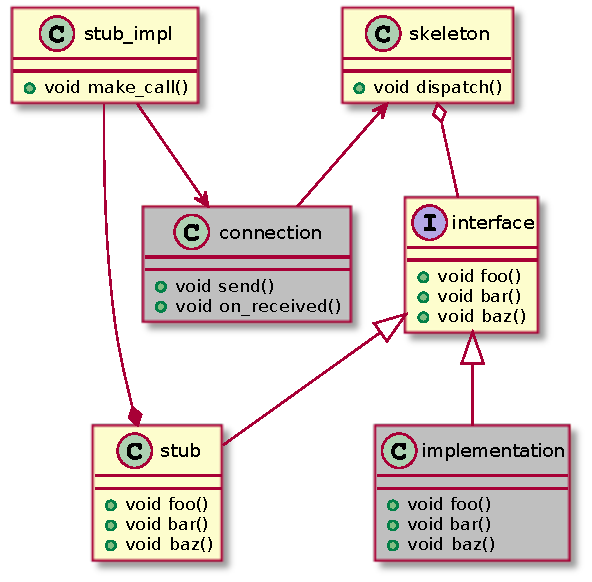
\includegraphics[
        width=0.65\textwidth,
        keepaspectratio
    ]{rpc_class.pdf}
    \end{minipage}
  }
\end{frame}
% ------------------------------------------------------------------------------
\begin{frame}
  \frametitle{Remote procedure calls}
  \framesubtitle{synchronous call sequence}
  \colorbox{lightgray}{
    \begin{minipage}{\dimexpr\textwidth\relax}
    \centering
    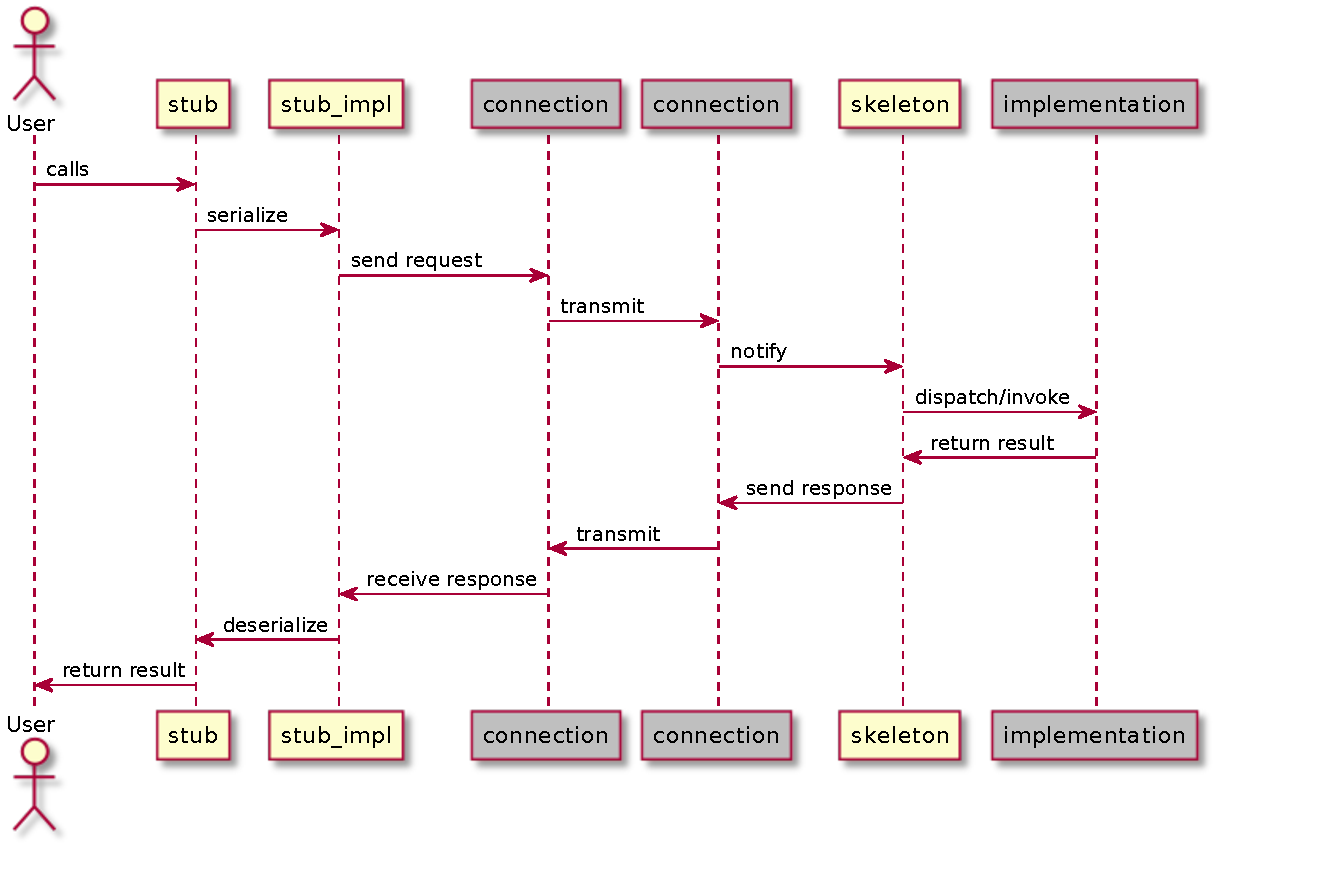
\includegraphics[
        width=0.9\textwidth,
        keepaspectratio
    ]{rpc_sequence.pdf}
    \end{minipage}
  }
\end{frame}
% ------------------------------------------------------------------------------
\begin{frame}[fragile]
  \frametitle{RPC stubs/skeletons}
  \framesubtitle{the interface}
  \begin{lstlisting}[language=c++2x,basicstyle=\small\ttfamily]
struct calculator {
    virtual float add(float, float) = 0;
    virtual float subtract(float, float) = 0;
    virtual float multiply(float, float) = 0;
    virtual float divide(float, float) = 0;
    virtual float negate(float) = 0;
    virtual float invert(float) = 0;
};
  \end{lstlisting}
\end{frame}
% ------------------------------------------------------------------------------
\begin{frame}[fragile]
  \frametitle{RPC stubs/skeletons}
  \framesubtitle{the stub}
  \begin{lstlisting}[language=c++2x,basicstyle=\footnotesize\ttfamily]
class calculator_stub : public calculator {
private:
    (*@\listinghl{rpc_stub_impl}@*) _impl;
public:
  float add(float l, float r) final {
    return _impl.(*@\listinghl{make_call}@*)(
      (*@\listinghl{mirror}@*)((calculator::add(l, r))), l, r);
  }

  float subtract(float l, float r) final {
    return _impl.make_call(
      mirror((calculator::subtract(l, r))), l, r);
  }

  float multiply(float l, float r) final;
  float divide(float l, float r) final;
  float negate(float x) final;
  float invert(float x) final;
};
  \end{lstlisting}
\end{frame}
% ------------------------------------------------------------------------------
\begin{frame}[fragile]
  \frametitle{RPC stubs/skeletons}
  \framesubtitle{the generic stub implementation\footnote{pseudocode}}
  \begin{lstlisting}[language=c++2x,basicstyle=\footnotesize\ttfamily]
class rpc_stub_impl {
  template <typename T>
  auto _deserialize(packet&, (*@\listinghl{type_identity}@*)<T>) -> T;
public:
  auto make_call(metaobject auto mo, auto&... args) {

    packet request;
    _serialize(request, mo, args...);
    packed response{_send_and_receive(request)};

    return _deserialize(
      response,
      (*@\listinghl{get_reflected_type}@*)(
        (*@\listinghl{get_type}@*)(
          (*@\listinghl{get_callable}@*)(
            (*@\listinghl{get_subexpression}@*)(mo)))));
  }
};
  \end{lstlisting}
\end{frame}
% ------------------------------------------------------------------------------
\begin{frame}[fragile]
  \frametitle{RPC stubs/skeletons}
  \framesubtitle{the skeleton interface}
  \begin{lstlisting}[language=c++2x]
struct rpc_skeleton {
  virtual void dispatch(
    packet& request,
    packet& response) = 0;
};
  \end{lstlisting}
  \begin{itemize}
    \item Could be plugged-into a network connection
    \item Handle incoming data
    \item After call is finished the connection can send the response
  \end{itemize}
\end{frame}
% ------------------------------------------------------------------------------
\begin{frame}[fragile]
  \frametitle{RPC stubs/skeletons}
  \framesubtitle{the skeleton implementation\footnote{pseudocode}}
  \begin{lstlisting}[language=c++2x,basicstyle=\scriptsize\ttfamily]
template <typename Intf>
class rpc_skeleton_impl : public rpc_skeleton {
private:
  std::unique_ptr<Intf> _impl;
public:
  void dispatch(packet& request, packet& response) final {
    const auto method_id{_get_method_id(request)};

    for_each(get_member_functions(mirror(Intf)),
      [&](auto mf) {
        if(_get_method_id(mf) == method_id) {
          auto params = (*@\listinghl{make_value_tuple}@*)(
            (*@\listinghl{transform}@*)((*@\listinghl{get_parameters}@*)(mf), (*@\listinghl{get_type}@*)(_1)));

          deserialize(params, request);
          auto result = (*@\listinghl{apply}@*)(mf, *_impl, params);
          serialize(method_id, result, response);
        }
    });
  }
}
  \end{lstlisting}
\end{frame}
% ------------------------------------------------------------------------------
\begin{frame}[fragile]
  \frametitle{\say{Smart} concept definition}
  \framesubtitle{featuring CTRE!}
  \begin{lstlisting}[language=c++2x,basicstyle=\footnotesize\ttfamily]
template <typename T>
concept very_smart_integer(*@\footnote{don't try this at home}@*) = (*@\listinghl{ctre_match}@*)<
  "((signed|unsigned) )?"\
  "((long long|long|short)( int)?|int)"
>((*@\listinghl{get_name}@*)(remove_all_aliases(mirror(T))));

auto add(
  very_smart_integer auto l,
  very_smart_integer auto r) {
    return l + r;
}
  \end{lstlisting}
  \begin{lstlisting}[language=c++2x,basicstyle=\small\ttfamily]
cout << add(1U, 2U) << endl;
cout << add(short(3), short(4)) << endl;
cout << add(21, 21) << endl;
cout << add(400ULL, 20ULL) << endl;
  \end{lstlisting}
\end{frame}
% - Conclusion -----------------------------------------------------------------
\section{Conclusion}
% ------------------------------------------------------------------------------
\begin{frame}
  \frametitle{Conclusions}
  \larger
  \begin{itemize}
    \item Reflection is {\em \larger fun}
    \item Reflection is {\em \larger useful}
    \item Reflection code can be readable
    \item Reflection code can be straightforward to write
    \item Reflection code doesn't need to look like punctuation-soup\footnote{
        for the most part}
    \item Reflection APIs can provide many non-trivial, reusable tools
  \end{itemize}
\end{frame}
% ------------------------------------------------------------------------------
\begin{frame}
  \frametitle{There are so many use-cases}
  \framesubtitle{details in other talks}
  \begin{itemize}
    \item Implementation of the {\em factory} pattern
    \item Auto-registering with script language bindings
    \item Generating GUIs for visualization and data input
    \item Serialization and deserialization
    \item Generating UML diagrams from code
    \item Generating DB system queries
    \item Fetching data from databases into C++ structures
    \item Parsing of configuration files
    \item Parsing of command-line arguments
    \item Mapping of URL arguments to function arguments
    \item \ldots
  \end{itemize}
\end{frame}
% ------------------------------------------------------------------------------
\begin{frame}
  \frametitle{Where does all this come from?}
  \larger
  \begin{itemize}
    \item The {\em Mirror} library
    \begin{itemize}
      \item primitive and sequence operations,
      \item algorithms,
      \item placeholder expressions,
      \item examples and use-cases\footnote{including bigger ones},
      \item integration with other projects\footnote{CTRE, rapidjson, chaiscript,
        sqlite3, etc.},
      \item \ldots
    \end{itemize}
    \item On top of the reflection TS implementation in \inlinecode{clang}
    \item There is much more than what fits into this talk
    \item See the reference (links below)
  \end{itemize}
\end{frame}
% ------------------------------------------------------------------------------
\begin{frame}
  \frametitle{Links, shameless plugs, etc.}
  \begin{itemize}
    \item {\em Reflection TS in \inlinecode{clang}} --
      \url{https://github.com/matus-chochlik/llvm-project}
    \item {\em The Mirror library repository} --
      \url{https://github.com/matus-chochlik/mirror}
    \item {\em The Mirror library reference (W.I.P.)} --
      \url{matus-chochlik.github.io/mirror/doxygen/}
  \end{itemize}
\end{frame}
% ------------------------------------------------------------------------------
\begin{frame}
  \frametitle{What's next for reflection?}
  \Large
  \begin{itemize}
    \item More \say{un-reflection}
    \item Code fragment splicing
    \item Splicing {\em \larger identifiers} depending on metaobjects\footnote{
        maybe even with custom formatting}
    \item Support for more use-cases
  \end{itemize}
\end{frame}
% ------------------------------------------------------------------------------
\begin{frame}
  \frametitle{That's all folks\dots}
  \centering
  \Huge
  Thanks for your attention.\\
  \Large
  Happy to answer any additional questions.
\end{frame}
% - Extras ---------------------------------------------------------------------
\section{Extras}
% ------------------------------------------------------------------------------
\begin{frame}
  \frametitle{There is more}
  \makebox[\linewidth][c]{
    \begin{minipage}{\dimexpr\textwidth\relax}
    \centering
    
\includegraphics[
        width=0.9\textwidth,
        keepaspectratio
    ]{extras.png}
    \end{minipage}
  }
\end{frame}
% ------------------------------------------------------------------------------
\begin{frame}[fragile]
  \frametitle{MOAR \say{smart} concepts!}
  \begin{lstlisting}[language=c++2x,basicstyle=\small\ttfamily]
struct excellent {
    void foo() {}
    void bar() {}
    void baz() {}
};
  \end{lstlisting}
  \vfill
  \begin{lstlisting}[language=c++2x,basicstyle=\small\ttfamily]
template <typename T>
concept has_foo_and_such = any_of(
  get_member_functions(mirror(T)),
  ctre_match<"foo|bar|baz">(get_name(_1)));
  \end{lstlisting}
  \vfill
  \begin{lstlisting}[language=c++2x,basicstyle=\small\ttfamily]
void foonction(has_foo_and_such auto) {
    cout << "this is excellent!" << endl;
}
  \end{lstlisting}
  \vfill
  \begin{lstlisting}[language=c++2x,basicstyle=\small\ttfamily]
foonction(excellent{});
foonction(std::string{}); // ERROR
  \end{lstlisting}
\end{frame}
% ------------------------------------------------------------------------------
\begin{frame}[fragile]
  \frametitle{Min/max enumerator value}
  \begin{lstlisting}[language=c++2x,basicstyle=\footnotesize\ttfamily]
auto min_enum = get_top_value(
  get_enumerators(_1),
  get_constant(_1),
  std::greater<>{});
  \end{lstlisting}
  \vfill
  \begin{lstlisting}[language=c++2x,basicstyle=\footnotesize\ttfamily]
auto max_enum = get_top_value(
  get_enumerators(_1),
  get_constant(_1),
  std::less<>{});
  \end{lstlisting}
  \vfill
  \begin{lstlisting}[language=c++2x,basicstyle=\footnotesize\ttfamily]
auto print_info = [&](auto me) {
  cout << get_name(me)
       << ":  min(" << enum_to_string(min_enum(me))
       << "), max(" << enum_to_string(max_enum(me))
       << ")" << std::endl;
};
  \end{lstlisting}
\end{frame}
% ------------------------------------------------------------------------------
\begin{frame}[fragile]
  \frametitle{Are enumerators bitfield bits?}
  \begin{lstlisting}[language=c++2x,basicstyle=\footnotesize\ttfamily]
const auto is_bitfield_enum =
  is_sorted(get_enumerators(_1), [](auto l, auto r) {
    if constexpr(has_type_trait<is_signed>(
      get_underlying_type(get_type(l)))) {
      return false;
    } else {
      auto to_underlying = [](auto e) {
        using U = underlying_type_t<decltype(e)>;
        return static_cast<U>(e);
      };
      return to_underlying(get_constant(l)) << 1U ==
             to_underlying(get_constant(r));
    }
  });
  \end{lstlisting}
\end{frame}
% ------------------------------------------------------------------------------
\begin{frame}[fragile]
  \frametitle{Are member functions sorted by name?}
  \begin{columns}
    \begin{column}{.65\textwidth}
      \begin{lstlisting}[language=c++2x,basicstyle=\footnotesize\ttfamily]
struct foo {
  int plus(int x) {
    return x;
  }
  int plus(int x, int y) {
    return x + y;
  }
  int plus(int x, int y, int z) {
    return x + y + z;
  }
  int minus(int x) {
    return -x;
  }
  int minus(int x, int y) {
    return x - y;
  }
};
      \end{lstlisting}
    \end{column}
    \begin{column}{.35\textwidth}
      \begin{lstlisting}[language=c++2x,basicstyle=\small\ttfamily]
struct bar {
  int a() {
    return 0;
  }
  int b() {
    return 1;
  }
  int c() {
    return 2;
  }
};
      \end{lstlisting}
    \end{column}
  \end{columns}
\end{frame}
% ------------------------------------------------------------------------------
\begin{frame}[fragile]
  \frametitle{Are member functions sorted by name?}
  \begin{lstlisting}[language=c++2x,basicstyle=\small\ttfamily]
const auto are_sorted_by_name = is_sorted(
  get_member_functions(_1),
  get_name(_1) < get_name(_2));

cout << are_sorted_by_name(mirror(foo))<< endl;
cout << are_sorted_by_name(mirror(bar))<< endl;
  \end{lstlisting}
  Output:
  \begin{verbatim}
  0
  1
  \end{verbatim}
\end{frame}
% ------------------------------------------------------------------------------
% ------------------------------------------------------------------------------
\end{document}
